% This is text associated with the open textbook "Open Electromagnetics"
% See immediately below for author, date
% This work is licensed under the Creative Commons Attribution-ShareAlike 4.0 International License. (CC BY SA 4.0) 
% To view a copy of the license, visit http://creativecommons.org/licenses/by-sa/4.0/

%ORB TITLE Conductance
%ORB AUTHOR 0        # S.W. Ellingson, Virginia Tech (ellingson@vt.edu)
%ORB DATE 20180806  # yyyymmdd
%ORB ABSTRACT Conductance at DC

\label{m0105_Conductance_DC} % <-- Must match name of this file and module directory name.  Don't mess with this!
\index{conductance|(}

Conductance, like resistance (Section~\ref{m0071_Resistance_DC}), is a property of devices. Specifically:
%
%ORB HIGHLIGHT
\begin{mdframed}[backgroundcolor=yellow!20,nobreak=true] 
Conductance 
\index{conductance!definition}
$G$ ($\Omega^{-1}$ or S) is 
the reciprocal of resistance $R$.
\end{mdframed}
%
Therefore, conductance depends on both the conductivity of the materials used in the device, as well as the geometry of the device.

A natural question to ask is, why do we require the concept of conductance, if it simply the reciprocal of resistance?
The short answer is that the concept of conductance is \emph{not} required; or, rather, we need only resistance \emph{or} conductance and not both.
Nevertheless, the concept appears in engineering analysis for two reasons:
%
\begin{itemize}
\item Conductance is sometimes considered to be a more intuitive description of the underlying physics in cases where the applied voltage is considered to be the independent ``stimulus'' and current is considered to be the response.
This is why conductance appears in the lumped element model for transmission lines (Section~\ref{m0029_Lumped-Element_Model}), for example.
\item Characterization in terms of conductance may be preferred when considering the behavior of devices in parallel, since the conductance of a parallel combination is simply the sum of the conductances of the devices.
\end{itemize}

%-------------------------------------------------------------------------

\index{transmission line!coaxial|(}

%ORB EXAMPLE
~\\ \begin{example} 
\begin{mdframed}[backgroundcolor=brown!20,linecolor=brown!20]\raggedright
Conductance of a coaxial structure.
\\~\\
Let us now determine the conductance of a structure consisting of coaxially-arranged conductors separated by a lossy dielectric, as shown in Figure~\ref{m0105_fCondCoax}.
The conductance per unit length $G'$ (i.e., S/m) of this structure is of interest in determining the characteristic impedance of coaxial transmission line, as addressed in Sections~\ref{m0029_Lumped-Element_Model} and \ref{m0143_Coaxial_Line}.

For our present purposes, we may model the structure as two concentric perfectly-conducting cylinders of radii $a$ and $b$, separated by a lossy dielectric having conductivity $\sigma_s$.
We place the $+z$ axis along the common axis of the concentric cylinders so that the cylinders may be described as constant-coordinate surfaces $\rho=a$ and $\rho=b$.

There are at least 2 ways to solve this problem.
One method is to follow the procedure that was used to find the capacitance of this structure in Section~\ref{m0113_Capacitance_of_Coaxial_Line}.
Adapting that approach to the present problem, one would assume a potential difference $V$ between the conductors, from that determine the resulting electric field intensity ${\bf E}$, and then using Ohm's Law for Electromagnetics (Section~\ref{m0010_Conductivity}) determine the density ${\bf J}=\sigma_s {\bf E}$ of the current that leaks directly between conductors. From this, one is able to determine the total leakage current $I$, and subsequently the conductance $G\triangleq I/V$.  
Although highly recommended as an exercise for the student, in this section we take an alternative approach so as to demonstrate that there are a variety of approaches available for such problems.
%%% TODO PROBLEM

The method we shall use below is as follows:
(1) Assume a leakage current $I$ between the conductors; 
(2) Determine the associated current density ${\bf J}$, which is possible using only geometrical considerations; 
(3) Determine the associated electric field intensity ${\bf E}$ using ${\bf J}/\sigma_s$;
(4) Integrate ${\bf E}$ over a path between the conductors to get $V$.
Then, as before, conductance $G\triangleq I/V$.

The current $I$ is defined as shown in Figure~\ref{m0105_fCondCoax}, with reference direction according to the engineering convention that positive current flows out of the positive terminal of a source.
%%% TODO Problem: It's worth noting that the opposite direction may be used for the reference direction as well, with the appropriate changes in sign throughout the rest of the work.
The associated current density must flow in the same direction, and the circular symmetry of the problem therefore constrains ${\bf J}$ to have the form 
%
\begin{equation}
{\bf J} = \hat{\bf \rho}\frac{I}{A}
\end{equation}
%
where $A$ is the area through which $I$ flows.  
In other words, current flows radially outward from the inner conductor to the outer conductor, with density that diminishes inversely with the area through which the total current flows.
(It may be helpful to view ${\bf J}$ as a flux density and $I$ as a flux, as noted in Section~\ref{m0101_Current_Distributions}.)
This area is simply circumference $2\pi\rho$ times length $l$, so
%
\begin{equation}
{\bf J} = \hat{\bf \rho}\frac{I}{2\pi\rho l}
\end{equation}
%
which exhibits the correct units of A/m$^2$.

Now from Ohm's Law for Electromagnetics we find the electric field within the structure is
%
\begin{equation}
{\bf E} = \frac{{\bf J}}{\sigma_s} = \hat{\bf \rho}\frac{I}{2\pi\rho l \sigma_s}
\end{equation}

Next we get $V$ using (Section~\ref{m0061_Force_Energy_and_Potential_Difference})
%
\begin{equation}
V = -\int_{\mathcal C}{ {\bf E} \cdot d{\bf l} }
\end{equation}
%
where $\mathcal{C}$ is any path from the negatively-charged outer conductor to the positively-charged inner conductor.
Since this can be \emph{any} such path (Section~\ref{m0062_Independence_of_Path}), we should choose the simplest one.
The simplest path is the one that traverses a radial of constant $\phi$ and $z$.
Thus: 
%
\begin{flalign}
V &= -\int_{\rho=b}^a{ \left( \hat{\bf \rho} \frac{I}{2\pi \rho l \sigma_s } \right) \cdot \left(\hat{\bf \rho}d\rho\right) }  \nonumber \\
  &= - \frac{I}{2\pi l \sigma_s } \int_{\rho=b}^a{ \frac{d\rho}{\rho}  }  \nonumber \\
  &= + \frac{I}{2\pi l \sigma_s } \int_{\rho=a}^b{ \frac{d\rho}{\rho}  }  \nonumber \\
  &= + \frac{I}{2\pi l \sigma_s } \ln\left(\frac{b}{a}\right)
\end{flalign} 

Wrapping up:
%
\begin{equation}
G \triangleq \frac{I}{V} = \frac{I}{ \left( I / 2\pi l \sigma_s \right) \ln\left(b/a\right) }
\end{equation}
%
Note that factors of $I$ in the numerator and denominator cancel out, leaving:
%
\begin{equation}
\boxed{
G = \frac{2\pi l \sigma_s}{\ln\left(b/a\right)}   
}
\label{m0105_eGcoax}
\end{equation}
%
Note that Equation~\ref{m0105_eGcoax} is dimensionally correct, having units of S $=$ $\Omega^{-1}$. 
Also note that this is expression depends only on materials (through $\sigma_s$) and geometry (through $l$, $a$, and $b$).
Notably it does \emph{not} depend on current or voltage, which would imply non-linear behavior.

To make the connection back to lumped-element transmission line model parameters (Sections~\ref{m0029_Lumped-Element_Model} and \ref{m0143_Coaxial_Line}), we simply divide by $l$ to get the per-length parameter:
%
\begin{equation}
\boxed{
G' = \frac{2\pi \sigma_s}{\ln\left(b/a\right)}   
}
\label{m0105_eGp}
\end{equation}
\end{mdframed}
%
\begin{figure}
\begin{center}
\pdftooltip{{  % note double braces
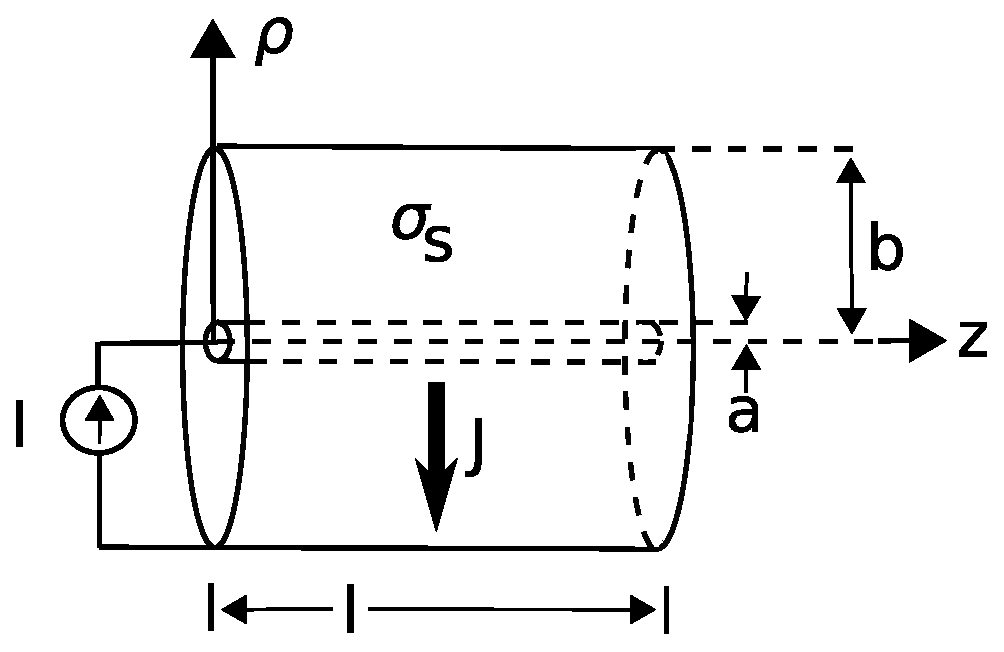
\includegraphics[width=2.5in]{modules/m0105_fCondCoax.eps}
}}{Coaxially-arranged conductor cylinders centered on the z-axis, with the smaller, inner cylinder having radius a, length l, and the larger, outer cylinder having radius b, length l. Current is shown flowing from exterior to interior. A vector, rho, extends from the middle of the inner cylinder upward. A large arrow in the middle of the cylinders points down, labeled bold J. The region between the cylinders has conductance sigma sub s.}
\end{center} 
% URL
%\centerline{\scriptsize 
%\copyright~\hyperref[m0105_fCondCoax_Credit]{Author} 
%\href{https://creativecommons.org/licenses/by-sa/4.0/}{CC BY~SA 4.0} 
%} 
\caption{
\label{m0105_fCondCoax}
Determining the conductance of a structure consisting of coaxially-arranged conductors separated by a lossy dielectric.
}
\end{figure}
\end{example}

%-------------------------------------------------------------------------
 
%ORB EXAMPLE
~\\ \begin{example} 
\begin{mdframed}[backgroundcolor=brown!20,linecolor=brown!20]\raggedright
Conductance of RG-59 
\index{RG-59}
coaxial cable.
\\~\\
RG-59 coaxial cable consists of an inner conductor having radius $0.292$~mm, an outer conductor having radius $1.855$~mm, and a polyethylene spacing material exhibiting conductivity of about $5.9\times 10^{-5}$~S/m.
Estimate the conductance per length of RG-59.

{\bf Solution.} 
From the problem statement, 
$a=0.292$~mm, 
$b=1.855$~mm, 
and $\sigma_s \cong 5.9\times 10^{-5}$~S/m.
Using Equation~\ref{m0105_eGp}, we find $G'\cong 200~\mu$S/m.

\end{mdframed}\end{example}

\index{transmission line!coaxial|)}

\index{conductance|)}
